\section{Mikrocontroller und eingebettete Systeme}

\subsection*{Aufbau und Hauptkomponenten}
Ein \emph{Mikrocontroller} ist ein kleiner Computer auf einem einzigen integrierten Schaltkreis, der eine zentrale Recheneinheit (CPU), Speicher und Ein-/Ausgabe-Peripherie enthält. Er ist für spezifische Steuerungsaufgaben konzipiert und bildet das Herz vieler eingebetteter Systeme. \emph{Eingebettete Systeme} sind spezialisierte Computersysteme, die als Teil eines größeren Geräts eine dedizierte Funktion erfüllen. Typischerweise integriert ein Mikrocontroller alle notwendigen Komponenten – CPU, Programmspeicher (meist Flash), Datenspeicher (SRAM), Timer, digitale/analoge I/O, serielle Schnittstellen usw. – auf einem einzigen Chip, sodass kein externes Unterstützungschip erforderlich ist. Dadurch können Mikrocontroller autark Geräte wie Sensoren und Aktoren steuern. \autocite{Microcontroller_vs_Microprocessor}

\begin{figure}[H]
	\centering
	\vspace{1em}
	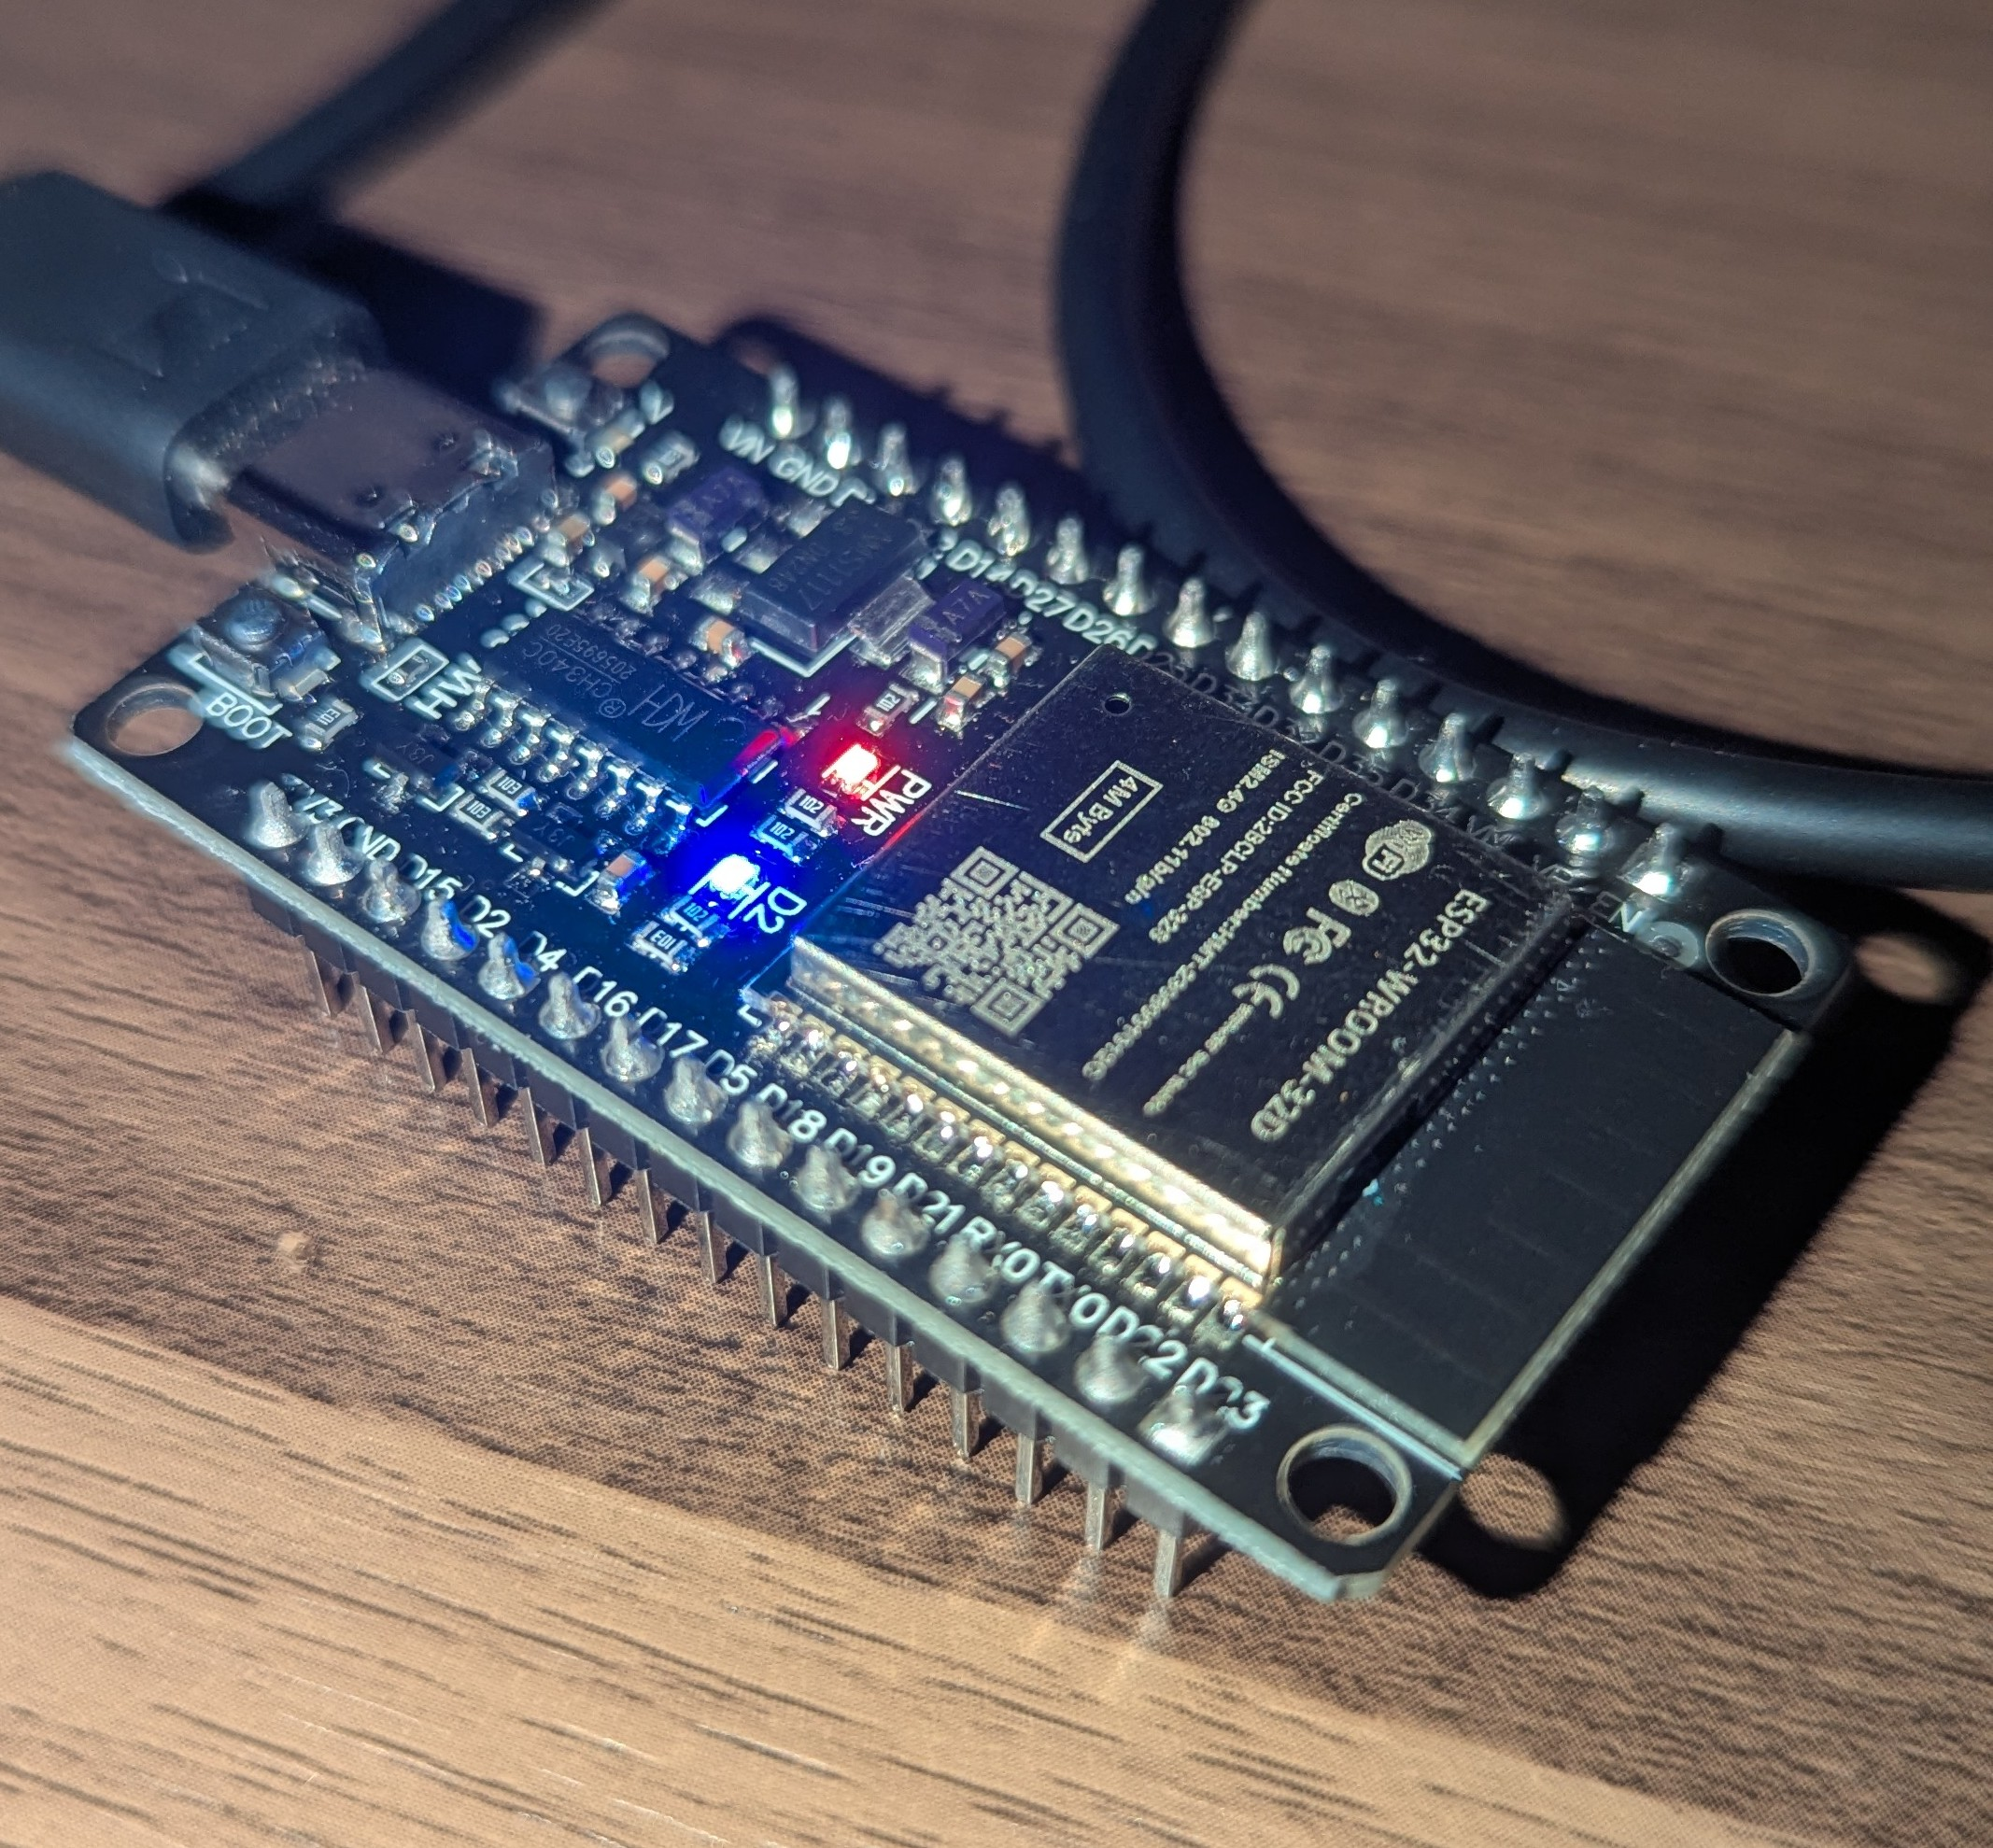
\includegraphics[width=0.5\textwidth, height=0.5\textheight, keepaspectratio]{./img/PXL_20250414_235020869.jpg}
	\caption{Bild eines ESP32 Mikrocontrollers}
	\label{fig:ESP32}
\end{figure}
\newpage

\subsection*{Energiemanagement}
In Heimautomatisierung und IoT-Anwendungen ist \emph{Energiemanagement} zentral, da viele Geräte batteriebetrieben oder dauerhaft aktiv sind. Mikrocontroller bieten verschiedene Low-Power-Modi (z.\,B. Schlafmodus, Tiefschlafmodus), in denen sie unbenötigte Komponenten abschalten oder deren Takt reduzieren, um Energie zu sparen. \autocite{energiesparen} Beispielsweise können Peripherien deaktiviert und durch \emph{Clock Gating} der Takt für inaktive Module angehalten werden, um den Verbrauch zu senken. \autocite{energiesparen} Moderne Techniken wie \emph{Dynamic Voltage and Frequency Scaling} (DVFS) passen zudem Versorgungsspannung und Taktfrequenz dynamisch an die aktuelle Rechenlast an. \autocite{energiesparen} Auf diese Weise lässt sich die Leistungsaufnahme minimieren, ohne die essenziellen Funktionen zu beeinträchtigen. Ein effizientes Energiemanagement verlängert die Batterielaufzeit und reduziert die Wärmeentwicklung – beides essenziell für sensorbasierte Haussteuerungen mit dauerhafter Betriebsbereitschaft.

\subsection*{Echtzeitverhalten}
Eingebettete Systeme zur Steuerung von Geräten im Smart Home unterliegen oft \emph{Echtzeit-Anforderungen}. \emph{Echtzeitsysteme} sind Systeme, die innerhalb vorgegebener Zeitgrenzen korrekt reagieren müssen; das zeitliche Verhalten ist Bestandteil der funktionalen Korrektheit. \autocite{echtzeit_grundlagen} Insbesondere ist die Korrektheit eines Echtzeitsystems nicht nur vom logischen Ergebnis, sondern auch vom physikalischen Zeitpunkt der Ergebniserzeugung bestimmt. \autocite{echtzeit_grundlagen} Man unterscheidet:
\begin{itemize}
  \item \textbf{Harte Echtzeit:} Eine Überschreitung der Deadline führt zu inakzeptablen Folgen (z.\,B. Gefährdung von Personen, Gerätebeschädigung). \autocite{echtzeit_grundlagen}
  \item \textbf{Weiche Echtzeit:} Timing-Verletzungen sind tolerierbar, führen aber zu Leistungseinbußen oder Qualitätsminderungen. \autocite{echtzeit_grundlagen}
\end{itemize}
In der Heimautomatisierung dominieren weiche Echtzeitanforderungen (z.\,B. Heizungsregelung), doch sicherheitsrelevante Funktionen wie Alarmanlagen oder Türschlosssteuerungen erfordern teilweise hartes Echtzeitverhalten. Entsprechend werden Mikrocontroller und ihre Software so ausgelegt, dass deterministische Reaktionszeiten eingehalten werden – etwa durch Einsatz von Echtzeitbetriebssystemen oder direktes Ausführen zeitkritischer Routinen ohne blockierende Aufrufe.

\subsection*{Interrupts}
Zur Realisierung eines responsiven Echtzeitverhaltens verwenden Mikrocontroller sogenannte \emph{Interrupts} (Unterbrechungen). Ein Interrupt ist ein asynchrones Signal, mit dem ein Peripheriegerät oder Sensor den Prozessor veranlasst, das reguläre Programm zu unterbrechen und eine vordefinierte \emph{Interrupt Service Routine (ISR)} auszuführen. Eine häufig zitierte Definition lautet: „Eine asynchrone Unterbrechung (IRQ) ist ein vom Prozessor-externen Umfeld generiertes Signal, das einen Zustand anzeigt und eine Behandlung durch den Prozessor anfordert. Dieses Signal ist nicht mit dem Programmlauf synchronisiert.“ \autocite{echtzeit_grundlagen}
\\
Durch Interrupts können externe Ereignisse (z.\,B. erkannte Bewegung) sofort bearbeitet werden, ohne auf die nächste zyklische Abfrage warten zu müssen. Dies ermöglicht \emph{ereignisgesteuerte Systeme}, die auf externe Signale in quasi Echtzeit reagieren. Alternativ existieren zeitgesteuerte (polling-basierte) Ansätze, bei denen der Mikrocontroller Sensoren in festen Intervallen abfragt. Interruptgesteuerte Designs haben den Vorteil minimaler Latenz, erfordern jedoch sorgfältiges Management (z.\,B. Priorisierung, Interrupt-Latenz), um Abläufe deterministisch und zuverlässig zu halten. In der Praxis werden häufig \emph{kombinierte Ansätze} genutzt: zeitgesteuerte Überwachung für reguläre Aufgaben und Interrupts für dringende Ereignisse.

\subsection*{I/O und Schnittstellen}
Mikrocontroller kommunizieren über diverse \emph{Ein-/Ausgabe-Schnittstellen} mit Sensoren, Aktoren und anderen Systemkomponenten. Sie verfügen über:
\begin{itemize}
  \item \textbf{Digitale I/O-Pins} zur Ansteuerung von Aktoren (z.\,B. Relais für Lampen) oder zum Erfassen binärer Signale (z.\,B. Fensterkontakte).
  \item \textbf{Analoge Eingänge} mit integrierten A/D-Wandlern zur Messung kontinuierlicher Größen (Temperatur, Helligkeit etc.).
  \item \textbf{PWM-Ausgänge} oder D/A-Wandler zur Ansteuerung analoger Aktoren (z.\,B. Dimmsteuerung, Motordrehzahl).
\end{itemize}
Gängige serielle Kommunikationsschnittstellen umfassen:
\begin{itemize}
  \item \textbf{UART (Universal Asynchronous Receiver Transmitter)} – für einfache Punkt-zu-Punkt-Kommunikation (z.\,B. mit Debugger, Bluetooth-Modul),
  \item \textbf{SPI (Serial Peripheral Interface)} – synchroner Hochgeschwindigkeitsbus für kurze Distanzen,
  \item \textbf{I²C (Inter-Integrated Circuit)} – Mehrpunktbus mit Adressierung, ideal für viele Sensorkomponenten,
  \item \textbf{CAN, USB, Ethernet} – für leistungsstärkere Anwendungen, z.\,B. in Gateways oder Fahrzeugtechnik. 
\end{itemize}
\autocite{Microcontroller_vs_Microprocessor}
Viele dieser Schnittstellen sind bereits im Mikrocontroller integriert. \autocite{Microcontroller_vs_Microprocessor} Auch sogenannte \emph{GPIOs} (General Purpose Input/Output) lassen sich flexibel als Ein- oder Ausgang programmieren. Die Vielfalt dieser Schnittstellen erlaubt es einem einzelnen Mikrocontroller, alle für eine Heimautomatisierungsaufgabe relevanten Sensoren und Aktoren direkt anzusteuern, ohne externe Steuerlogik. Die \textbf{korrekte Auswahl und Konfiguration} (z.\,B. Pull-up-Widerstände bei I²C, Bus-Timing, Interruptsteuerung bei UART) ist entscheidend für die Funktionssicherheit des Systems.

\subsection*{Abgrenzung zu System-on-Chips (SoCs)}
Der Begriff \emph{System-on-Chip} (SoC) überschneidet sich funktional mit dem des Mikrocontrollers, bezeichnet jedoch im weiteren Sinne einen integrierten Schaltkreis, der ein vollständiges elektronisches System auf einem Chip vereint. Mikrocontroller können als spezialisierte SoCs betrachtet werden, die primär einen Mikroprozessor mit Speicher und Basisperipherie für Steuerungsaufgaben enthalten.
\\
Im Unterschied dazu integrieren klassische SoCs zusätzliche leistungsfähige Komponenten wie GPU, DSP, drahtlose Kommunikationsmodule (WLAN, LTE), externe Speicheranbindung sowie komplexe Betriebssysteme (z.\,B. Linux, Android). Sie finden sich typischerweise in leistungsfähigen Smart-Home-Zentralen oder Gateways, die Daten aggregieren und komplexe Anwendungen wie Spracherkennung oder Cloud-Anbindung ausführen.
\\
Allgemein gilt: „Ein System-on-Chip ist ein vollständiges elektronisches System auf einem einzigen Chip, der eine Vielzahl von Funktionen ausführen kann.“ Mikrocontroller hingegen sind kompakter, energieeffizienter, günstiger und auf spezifische Aufgaben optimiert. Typische Flash-Größen liegen im Bereich von einigen Kilobyte bis wenigen Megabyte. \autocite{SoC}
\\
\paragraph{Fazit:} In der Heimautomatisierung finden sich beide Technologien: \textbf{Mikrocontroller} in Sensor- und Aktormodulen (z.\,B. ein Feuchtigkeitssensor mit Funkmodul) und \textbf{SoCs} in Smart-Home-Hubs und Gateways, die zentrale Logik und Kommunikation übernehmen.
